\documentclass[12pt,a4paper,fleqn]{article}
\usepackage{rmpackages}																% usual packages
\usepackage{rmtemplate}																% graphic charter
\usepackage{rmexocptce}																% for DS with cptce eval

%\cfoot{} 													% if no page number is needed
%\renewcommand\arraystretch{1.5}		% stretch table line height

\begin{document}
\normalem % makes emphasize italic again

\begin{header}
Défi astrophysique -- Spaghettification
\end{header}

\begin{multicols}{2}
\begin{center}
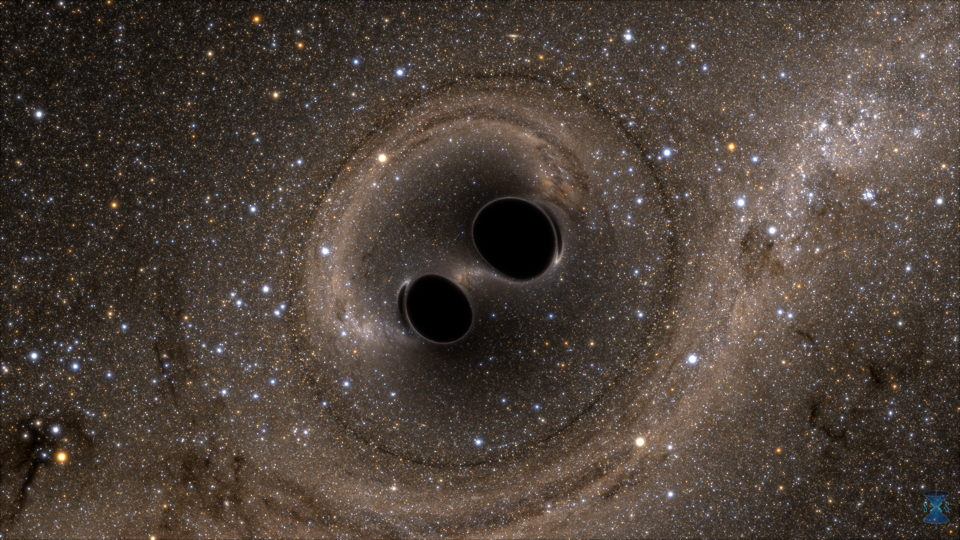
\includegraphics[width=\linewidth]{images/blackhole_gw150914.jpg}
\end{center}

L'existence des trous noirs a été postulée il y a près d'un siècle suite aux travaux d'Einstein sur la théorie de la relativité générale.
Cette hypothèse a été source de nombreux débats dans la communauté scientifique et elle n'a pu être vérifiée que récemment : pour des objets astronomiques, ils sont très petits et ils n'émettent pas de lumière.
Ils ont donc longtemps échappé à nos détecteurs, aussi perfectionnés soient-ils.
\end{multicols}

L'image ci-dessus est une vue d'artiste de deux trous noirs, quelques instants avant qu'ils ne fusionnent, le 14 septembre 2015.
Ci-dessous, à gauche, on voit le résultat d'un simulation réalisée par Jean-Pierre Luminet en 1978 : c'est la première représentation réaliste d'un trou noir.
À droite, il s'agit de la première photographie d'un trou noir, réalisée en 2019.

\begin{center}
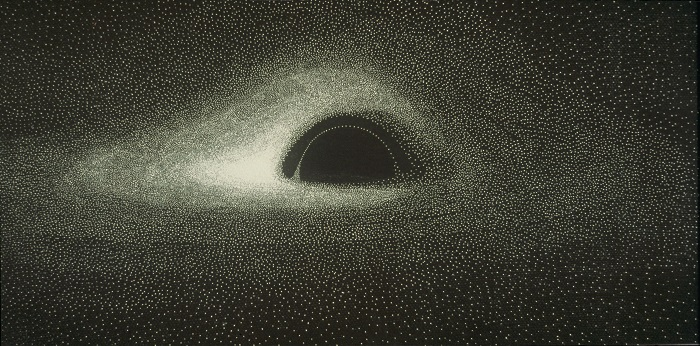
\includegraphics[height=140pt]{images/blackhole_luminet.jpg} \hfill
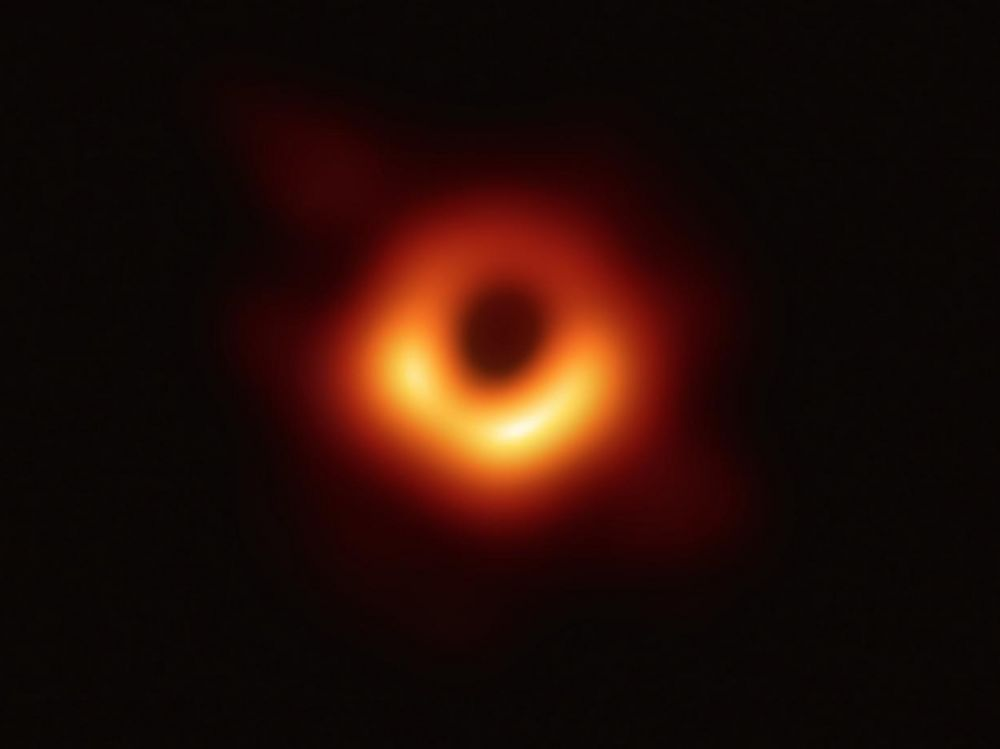
\includegraphics[height=140pt]{images/blackhole_photo.jpg}
\end{center}

Au voisinage d'un trou noir, des phénomènes étranges se produisent.
La \textbf{spaghettification}, aussi appelée \og \textbf{effet nouille} \fg{} est l'un de ces phénomènes.

\section*{Approche \og naïve \fg{} de la spaghettification}

Imaginons qu'un astronaute aventureux s'approche de la \og surface \fg{} d'un trou noir, les pieds dirigés vers le centre du trou noir. \footnote{On parle plutôt de l'horizon des évènements d'un trou noir.}
On suppose que les pieds de l'astronaute sont au niveau de la surface du trou noir.

\paragraph{Données}
\begin{center}
\begin{tabular}{ll}
Constante gravitationnelle & $G = \qty[per-mode=power]{6.67e-11}{\meter\cubed\per\kilogram\per\second\squared}$ \\
Masse du Soleil & $M_\odot = \qty{2e30}{\kilogram}$ \\
Masse du trou noir & $M = 60 \times M_\odot$ \\
Rayon du trou noir & $r = \qty{177}{\kilo\meter} $ \\
Masse des pieds d'un astronaute & $m = \qty{5}{\kilogram}$ \\
Masse de la tête d'un astronaute & $m = \qty{5}{\kilogram}$ \\
Taille d'un astronaute & $h = \qty{1.80}{m}$
\end{tabular}
\end{center}

Pour les applications numériques, on peut utiliser la calculatrice évidemment, mais aussi python en allant sur \href{https://www.lelivrescolaire.fr/outils/console-python}{https://www.lelivrescolaire.fr/outils/console-python}.

\begin{enumerate}
\item Sans soucis d'échelle, faire un schéma.

\item Calculer la force d'attraction gravitationnelle exercée par le trou noir sur les pieds de l'astronaute.

\item De même, calculer la force d'attraction gravitationnelle exercée par le trou noir sur la tête de l'astronaute.

\item Commenter les résultats obtenus et proposer une interprétation à la spaghettification.
\end{enumerate}

Pour aller plus loin, la vidéo de l'excellent David Louapre : \href{https://youtu.be/TdnER8AeIdw}{https://youtu.be/TdnER8AeIdw}.

\paragraph{Remarque :}
Il s'agit bien ici d'une approche naïve du phénomène : les trous noirs sont des objets atypiques qui ne sont pas bien décrits par la physique classique.
En particulier, très proche du trou noir, le modèle de la force d'attraction gravitationnelle vu en cours n'est plus valide, même s'il donne ici une bonne idée du phénomène.
Il faut utiliser des modèles plus élaborés pour obtenir des résultats fiables.
Mais ça, c'est le domaine de la relativité générale...

\end{document}